
\section{Clustering Comparison}
The three representatives were, as initially mentioned, chosen from each 
classical branch of clustering algorithm. The results more or less confirm
what is expected from the theoretical background, and enhances the 
conviction of the suitability of different algorithms.

\subsection{Performance}
When comparing the run-time of the three assessed algorithms by 
consulting figures~\ref{fig:moment-runtime-scatter} 
and~\ref{fig:day-runtime-scatter}, it is clear that CLARANS is 
significantly slower than DBSCAN, which in its turn generally
performs a bit slower than SLINK. These plots confirm the theoretical time 
complexities, with CLARANS being slowest.
%, by \ordo{bla} for each time the inner algorithm is run. 
As per recommendation of \citeauthor{CLARANS},
authors of the article \citetitle{CLARANS}, this 
inner algorithm is then run several times for different numbers of desired 
clusters $k$ in order to find the most natural number $k_{nat}$. The 
assessment in each step is done by calculating the Silhouette coefficient 
for the computation, and the $k$ producing the best coefficient is elected 
as $k_{nat}$, with the belonging computation. Each Silhouette run is done 
at \ordo{n^2}, yielding a total time complexity of \ordo{n^3} - \ordo{n^5},
depending on whether the clustering parameters $num\_local$ and $max\_neighbour$
rely on the number of data points or not. 

SLINK and DBSCAN performs similar time-wise, both depicting a 
time-complexity of \ordo{n^2}, with different coefficients in front of the 
expression. 

\begin{figure}[ht]
    \centering
    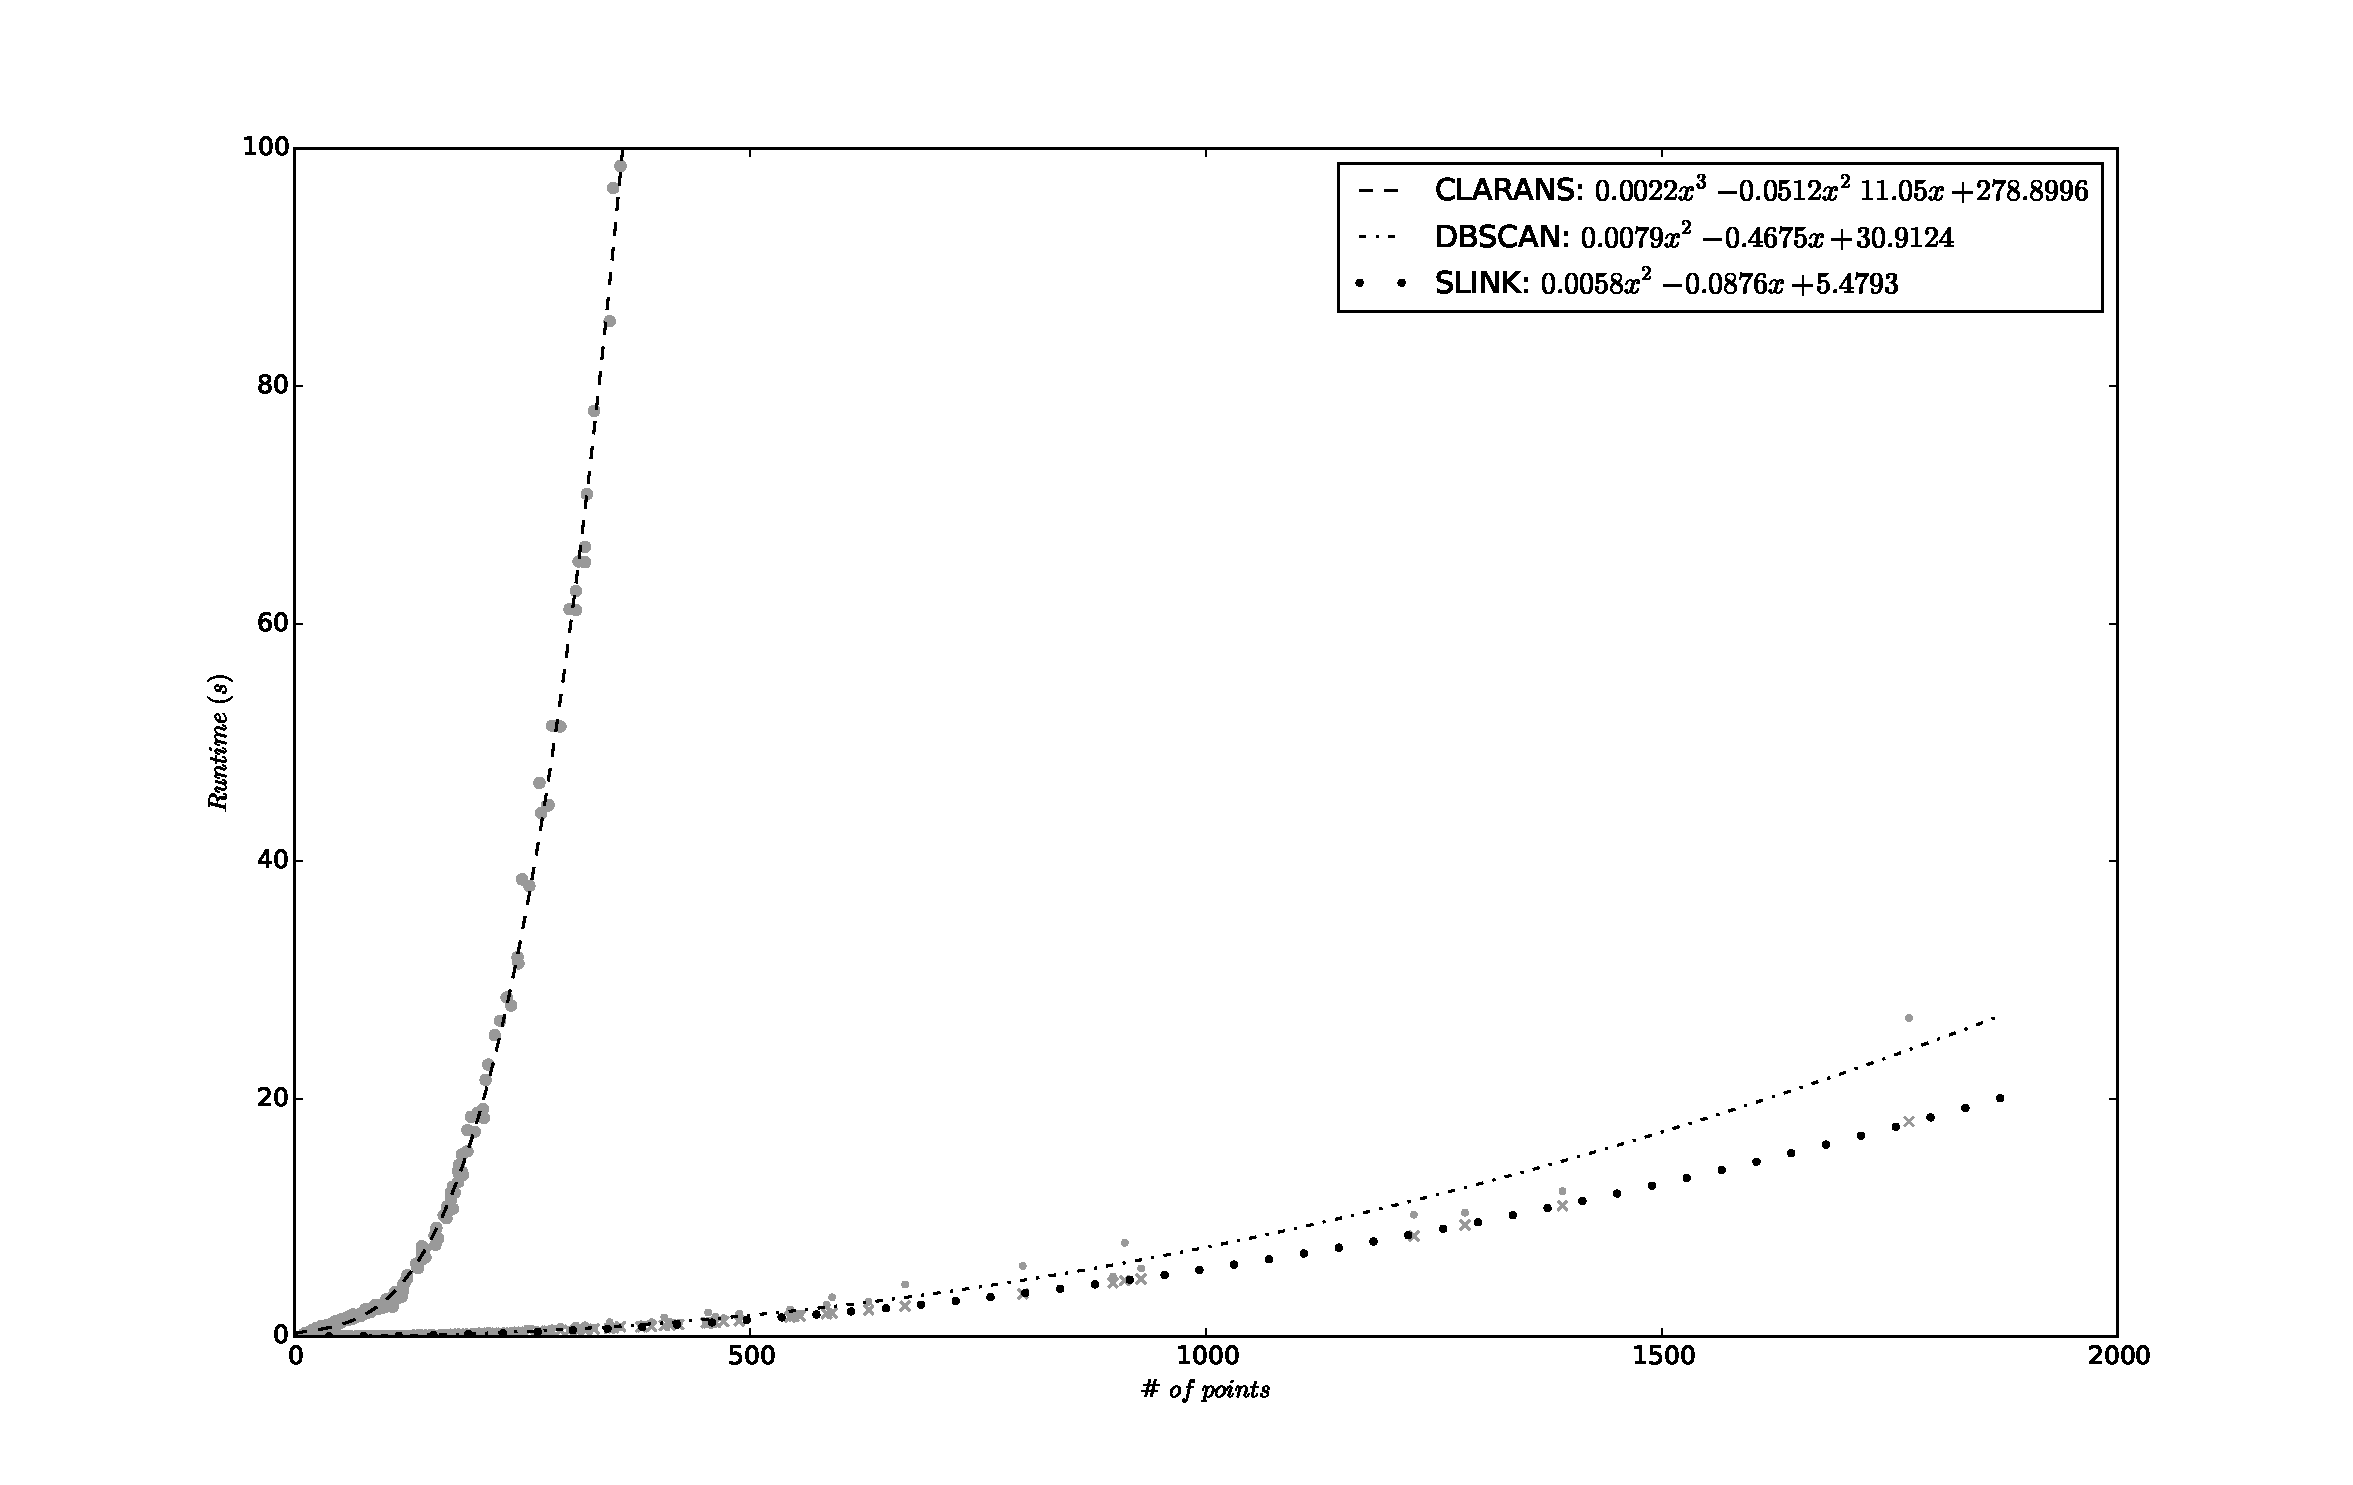
\includegraphics[width=0.9\textwidth]{plots/time_trendlines.pdf}
    \caption{Scatterplot of timestamps including trend lines.
    \label{fig:time-trendlines} }
\end{figure}

Using the polynomial fit for assessing \emph{trend lines} together with the 
observed data, coefficients for the polynomials are found yielding the trend 
lines as follows:
\begin{equation}
    \label{eq:trendline-equations}
    \begin{split}
        y_{CLARANS} &= 0.0022x^3 + 0.0512 x^2 +  11.05 x + 278.9 \\
        y_{DBSCAN}  &=           + 0.0079 x^2 + 0.4675 x +  30.9 \\
        y_{SLINK}   &=           + 0.0058 x^2 + 0.0876 x +   5.5
    \end{split}
\end{equation}
Plotting these along with the observed data is done in 
figure~\ref{fig:time-trendlines}, which makes the results seem feasible. 
It is likely to assume that these time complexities will hold for even 
larger numbers as well. 

It is worth noting that the region query algorithm used for DBSCAN is 
currently based on exhaustive search done in \ordo{n}, which leaves DBSCAN 
with a time complexity of \ordo{n^2}. A more rigid look up algorithm based 
on some R*-tree approach performing in \ordo{log(n)} should produce a 
somewhat faster result\footnote{
    Attempts were made at implementing this via RethinkDB:s spatial 
    queries, but unsuccessful as a mean of improving running time 
    efficiency loss. This is probable due to that RethinkDB is a database 
    focused on being distributed, yielding a time loss when querying the 
    database $n$ times. A faster approach was just to keep all data points 
    in memory. }.
An alternative to this if larger data sets are considered, is by either 
constructing some spatial index such as an R*-tree and inserting the data 
in it before performing spatial queries. \citeauthor{rtree-bulk-insert} 
did show that a bulk insert construction takes less than \ordo{n^2} 
time, and this spatial index implies a look up time of \ordo{ \log{n} }. 
Many databases already contain such indexes, and thus such queries can 
be done with a well considered database choice with simplicity \cite{rtree-bulk-insert}.

\subsection{Quality - Silhouettes}
Silhouettes are a measurement primarily for partitioning methods, and was 
originally developed with PAM and CLARA in mind by the authors 
\citeauthor{silhouettes} et al. An implicit assumption made, or a fact that is 
simply not considered, is that spatial points can be unassigned to clusters. 
The interpretation of Silhouettes here is simply not to treat these points 
and therefore, no evaluation of whether disregarding a point as noise is a 
good decision or not is taken into account.

Looking at figures~\ref{fig:clarans-silhouette}, \ref{fig:dbscan-silhouette} 
and~\ref{fig:slink-silhouette},
and taking the mean values depicted under each figure into account, it is 
clear that CLARANS produces the most qualitative clustering according to 
the criterion of maximizing the Silhouettes. This is expected, as the 
entire algorithms aim is to use the obtained Silhouette coefficients as 
feedback for how the algorithm is performing and which $k_{nat}$ to choose.

DBSCAN aims to eliminate bad clustering by regarding the entire observed 
Moment or data set as an activity. For the sake of being unbiased, a 
single detected cluster is awarded a Silhouette coefficient value of $0.5$,
which is why the algorithm produces that many clustering with the value of 
$0.5$. It has also the ability, unlike both CLARANS and SLINK, to disregard 
points as noise. Glancing at figure~\ref{fig:dbscan-vs-clarans} 
and~\ref{fig:dbscan-vs-slink} shows that DBSCAN generally produces few 
clusters given the set cluster parameters. This is desired, as we would not 
like a day to be divided into too many activities, and that a certain time 
should be spent at a certain location to deem it as an activity. 
Often for few data points, this setup yields a single cluster, disregardful 
of the Silhouette coefficient, which seems feasible as well as desirable.

SLINK produces poor clustering as well with regard to Silhouettes, partly 
because of the simple criterion on which the splitting is done. Unlike 
DBSCAN, it does not grant the ability to not use all the data points in the 
clustered result. During long, extended data sets right on the border of the 
limit value of breakpoints, a lot of clusters that are not very coherent will
be detected, leading to many clusters and to a poor clustering result. 

Taking one step back and evaluating the evaluation itself, it would seem like 
Silhouettes are not very suitable as a metric for comparing different 
clustering methods. However, it is one of few that is applicable 
at all regardless of which method is used, and therefore it is useful. One 
has to consider of course that the produced result is not easily interpretable, 
and requires prior knowledge about the algorithm being 
evaluated as well as insight in Silhouettes; how they are defined and some 
experience in how they behave when encountering different clustering. 
Given this, I argue that Silhouettes can be useful in a general 
manner and for a broader number of clustering applications, granted that 
one is familiar with the behaviour of Silhouettes. It serves as an aid to 
further evaluate why an algorithm performs as it does, and calls for 
another step of analysis. It is worth noting that a bad Silhouette score 
does not necessarily mean a bad clustering algorithm, it just means it is 
not optimized for this particular method.

\subsection{Produced Clusters}
Figure~\ref{fig:dbscan-vs-clarans}, \ref{fig:dbscan-vs-slink} 
and~\ref{fig:clarans-vs-slink} makes it very clear that different clustering
methods produce a different amount and different types of clusters. 

Generally, DBSCAN and CLARANS produce somewhat similar amount of clusters. 
This is due to that DBSCAN is not prone to produce many clusters given the
current clustering parameters, with $minPts$ set to $10\%$ of the data 
points, the absolute maximum number of clusters that is possible to obtain
is 10. In a similar manner, CLARANS is only able to produce at most 
$5$ clusters due to its limit set on the tests for $k_{nat}$. The produced
clusterings therefore does not differ very much in amount.

SLINK on the other hand tends to produce a lot more clusters in larger data
sets (as can be seen in both figure~\ref{fig:dbscan-vs-clarans} 
and~\ref{fig:clarans-vs-slink} where the number of clusters SLINK detects
diverges from the other algorithms more as the size of the data set increases). 
This is due to it's inability to disregard points as noise, while
bound to the same cutoff condition as DBSCANs $\epsilon$, yielding a lot
of small clusters containing a small number of points. Removing these would
be trivial in order to find remove noisy outliers with SLINK as well, but 
it would not serve any more comparison purposes than that.

\subsection{Large vs Small Data Sets}
Although CLARANS was specifically designed for working on larger data sets, 
both SLINK and DBSCAN outperforms CLARANS in the different sizes tested. 

As DBSCAN and CLARANS has an upper bound on the number of clusters that they
are able to detect in this instance as well, the results does not differ 
very much from the small data set. SLINK follows its previous trend 
with detecting even more clusters, since it is more flexible in its approach
on where to cut off its dendrogram into clusters.

\subsection{Method-specific qualities}
Different clustering methods have different qualities to take into account, 
both from a life-logging perspective, and with regard to finding different
types of clusters. 

CLARANS was built to maximize the Silhouette coefficient, and is useful for
finding clusters in very large data sets, especially large enough to not 
fit into the memory of the machine performing the clustering. Not keeping all
data points in memory would be a drawback for the other algorithms (granted 
that DBSCAN keeps its exhaustive search for nearby regions), but as it is 
randomized, clusters must be well-defined as well in order for it to locate 
them. This can be due to poor start-seed selections, meaning that the node 
chosen as a starting node is not very well spread out.
There exist methods for introducing starting seeds in partitioning
algorithms, usually with k-means being the target, but could applicable in 
this scenario as well. 
%When this is employed, the following results can
%be obtained following the same tests as above:

DBSCAN is easy to configure when working with activities and when following
equation~\ref{eq:minPts_eps_condition}, as one only needs to define 
how many data points are required for a series of samples to be considered
an activity. Disregarding outliers\footnote{
    An outlier is a data point that is distant from the other data points
    with regard to the distance function being used.
} is useful too, and making a qualitative
estimate of where the activity has taken place falls naturally. 
However, a decent knowledge about the size and characteristics of the 
assessed data set is necessary in order to get the desired result, and
clusters of varying densities are hard to distinct.  
Although the condition for selecting a good $\varepsilon$ and $minPts$ works
well with determining activities in a single cluster, it is not as 
accurate with higher number of data points and an expected higher number
of clusters. This since $minPts$ is set to contain a $10\%$ fraction of the total
points in the series to regard it as significant. A lower bound is also 
specified for this, and increasing DBCSANs performance of detecting more
clusters in bigger data sets could be accomplished by introducing an 
upper bound as well. 

SLINK is very customizable, as the splitting criterion defines which 
clusters are obtained. This would allow for more strict clustering
distinction, for instance by allowing time to a significant member in the 
distance function, and thus allowing finding of breakpoints in the time-line, 
and performing more strict clustering than DBSCAN.
SLINK also produces a hierarchical result. 
This hierarchical result is especially useful when multiple criteria 
need to be weighed in, and when allowing the result to be merged again or
split further without re-running the entire algorithm. 

\subsection{Desired Clusters}
From a life-logging point of view, there seem to be two different approaches
to what is a desired cluster to detect. 

One way, activity detection is of main interest and the output does not 
necessarily need to be in any specific form. What is desired is an estimate
of a location, time of stay and other similar data which will be used for 
classification or activity detection. It is more important that this produces
data that is neatly wrapped up and easy to present or use at a later step. 
This is the method used in the classification step of this thesis, when 
attempting to detect different activities. 

The alternative is that clustering in some hierarchy is required, where 
attributes are subordinated one another to perform division of data into 
smaller, ordered sets of data. This is what Narrative uses for dividing 
long series of images, into Moments (although, position or accelerometer
is currently not involved in this, only color data from images and timestamps 
are used for this clustering). Everything in this clustering is subordinated 
time, as Moments by Narratives definition is required to be coherent series 
of images. This calls for differently defined clusters, and thus differently
behaving clustering algorithms.

\section{Proof-of-Concept}
The proof-of-concept implementation conducted in this thesis adds components such
as clustering and classification to an already defined pipeline. The result of 
this implementation is presented earlier in this report, but the order of elements
in this already defined pipeline can be discussed. 

Long photo sequences are currently being divided into Moments solely based on 
timestamps and image analysis. It is at this point one would like to perform 
geo-spatial clustering if applicable, in order to get more natural Moments\footnote{
    The reason that no positional data is considered yet at this stage from 
    Narratives point of view is that no GPS points is available yet when the 
    \emph{Momentification} is done. This is produced later in the pipeline by 
    signal processing and by consulting servers for satellites positions. To 
    perform geo-spatial clustering in Narratives Momentification, this has to
    be addressed first. 
}. 
One might regard the existing implementation as a naive clustering algorithm, where 
introducing spatial data in the algorithm just increases the dimensionality, but
also the possibility of less artificial clusters. 


\section{Classification of Moments}

\subsection{Assessed Data Set}
As mentioned earlier, only employees were involved in the testing of the 
classification algorithm. It is feasible that employees of a company making
a certain life-logging device might utilize it another manner than the common 
user, which might have caused somewhat skewed results, but such that should
be sufficient for this thesis purposes.

\subsection{Possible Pitfalls}
As table~\ref{table:classification-values} witnesses of, the initial 
classification performs 
rather poorly, with each classification assignment except for the 
movement category only barely produced better 54\% correct 
approximations. There are many causes of this behaviour, and some 
being corrected led to  big improvement:

\begin{itemize}
\item The small sample for the algorithm to learn of was not sufficient, 
    and priors were not skewed enough to fit the model parameters to
    there correct location. This could have been prevented with a much
    bigger sample size. 
\item The sample for the learning algorithm were not diverse enough, and
    taken from a single user. Referencing 
    table~\ref{table:user-wise-mean-grade} it the mean value of users 
    assessments are widely varying. This can of course be a result of the
    users preferences while grading, but it also hints that the model 
    parameters are somewhat user-specific. For instance, a certain user 
    might move around more than another user while walking, therefore
    requiring somewhat different thresholds. Given this assumption, data
    from a small group of users will not reflect the entire population 
    of users, yielding skewed model parameters. 
\item The assigned probability distribution might not be suitable for the
    actual distribution, and thus the expert failed at the first attempt.
\end{itemize}

The model was simple and loosely defined upon assumptions, that might
prove more or less accurate. A model behaving incorrectly after many
learning attempts is probably an inaccurate model, but this should be
accommodated by updating ones model after observing its performance
in a true Bayesian manner.

The original intent of introducing such a model was for it to be 
simple and general enough to evaluate the method itself rather than
how this model would apply to Narratives employees and their Moments. 
Glancing ahead at the second attempt, it seems as the method holds.

\subsection{False Positives and Negatives}
Table~\ref{table:false-values-vs-grades} shows the correlation between
users grades for an entire activity classification, where the false 
negatives outweigh the number of false positives. Naturally, it seems 
more appealing for a user to receive a false negative rather than 
a false positive, implying that nothing special happened instead of 
saying something special happened while it did not. 

While the survey does not contain enough samples to statistically verify
this conclusively, it seems as a higher amount of false negatives is 
tolerated before lowering the grade of a classification, while false
positives are not tolerated at all. This backs our statements of false
positives being less appreciated. 

Given this information, one should focus on making an application that 
is less likely to produce a classification with greater semantic 
significance, as users seem more forgiving as towards missing out on 
classifications. As previously intended, assigned classes that are 
not semantically charged, which are assumed to be:
\begin{itemize}
    \item \emph{Alone} in the Social category.
    \item \emph{Off Hours} in the Working category.
    \item \emph{Stationary} in the Movement category.
    \item \emph{Indoors} in the Indoors category. 
\end{itemize}
should then not at all be shown to the end user, as they do not produce
enough value.

The scenario above applicable when the intention is to show the 
classifications to the end users. When the target instead is statistical
classification, for example in order for a company to determine the 
amount of activities its users engage in outdoors, these semantically 
charged notation is of less importance, as an overview of a whole group
is of greater interest than being correct in every individual case. 

\subsection{Second Attempt}

Analysis of the movement parameter is satisfactory, as it has three
possible outcomes and still manages to produce the best accuracy.

Relearning based on the new values allow a better fit for the observed
values, which are bound to be more diverse than samples from a single
user, as well as being a better quantity.

Looking at the results of the first attempt along with the number of
false positives and false negatives in table~\ref{table:classification-values} 
and table~\ref{table:false-values-before}, respectively, it is clear
that the categories \emph{Working} and \emph{Indoors} are not balanced.
Given that \emph{Working} depends on \emph{Indoors} (consulting 
figure~\ref{fig:bayes-network}), it seems logical in a first step to 
change \emph{Indoors}. By manually lowering the threshold of the 
model parameter (which was somewhat misplaced due to huge variance 
in the area-distribution), the results in table~\ref{table:classification-values} 
and table~\ref{table:false-values-before} were obtained.

Along with this, a relearning process is made where the percentages of 
the other assignments are somewhat improved, however not very 
significantly. Of course, this introduces a bias when the assessed data
is the same as the learned data, but given the sample size other tests
are not possible. This only illustrates the need of a larger data set 
for learning parameters, and the models influence in getting a faster
convergence towards correct classification.

This signals that a model error is present in the \emph{Indoors}-parameter,
and a model change should be done. In a Bayesian manner, preserving 
uncertainty is desired, and therefore introducing a second model
parameter denoting if the activity has any positional points could be
introduced. If this is the case, the area threshold is used, while 
otherwise, the original distribution of the \emph{Indoors} Bernoulli
variable is kept, thus preserving uncertainty.

\subsection{Iterative Process}

A way of looking at this attempt is simply as one stage of an iterative
process. In order for a sound model to develop with rigid model 
parameters several attempts seem to be required, and the first steps
of this process shows promise. It is also worth noting that the model
was initially predicted to not be too correct, as it was a simple 
version in order to evaluate the process and not the model. For a 
real-world implementation more analysis is definitely required in order
of creating more accurate predictions.

It has been shown that a learning step as well as a manual refinement of 
the model parameters result in a significant improvement. This is also
an example of how it is possible to go from a simple model producing 
mediocre results, to a more complex and targeted model towards more
specific problems.

\section{Big Data Ethics}

\subsection{What is Big Data?}

\begin{displayquote}
    ``Common definitions of the popular phrase for the phenomenon 
    “big data” are based on distinctions between the capabilities 
    of legacy database technologies and new data storage and 
    processing techniques and tools such as Hadoop clusters, 
    Bloom filters, and R data analysis tools. Big data is data too 
    big to be handled and analyzed by traditional database protocols
    such as SQL (which makes big data a term that  may evolve over 
    time; what is now big data may quite rapidly become small).''
    - \citeauthor{ethics-of-big-data}, author of 
    \citetitle{ethics-of-big-data} \cite{ethics-of-big-data}.
\end{displayquote}

What we particularly focus on in this thesis is just not the size,
but the applicability to make assumptions and draw conclusions based
on the observed user data. This is often the case for life-logging
devices, and cause for both use and abuse.

\subsection{Making Revenue}
Big data is a relatively new subject, or at least the extent of how it is used. 
Many companies are being able to make revenue on "free" services, which are free 
in the sense that the end user is the product. Mapping demographics and studying 
user behavior is becoming more and more a source of power for big data companies.
There are clearly different business models for the service providers, one being 
free-of-charge while collecting information about customers behaviours, the other 
being the classical approach of charging the end user for a service while not 
mining information about the user.

Simplified, it is two different payment methods for the users (while 
it might not be clear to the users themselves). The payment either comes
in the form of money, or utilizing your data, with various steps 
between. 

In any form - companies are not in the business of harming their customers,
so the customers are not the sole potential victims. As the amount of 
data increases, so does the need to protect the data and store it in a 
safe manner by the service provider. The more variate data that needs
to be stored in different ways, the more security holes need to be shut 
\cite{ethics-of-big-data}.

\subsection{An Ethics Code}

The need for an ethics code, or guidelines to follow when utilizing big data
computing is increasing with the number of companies engaging in the business.
\citeauthor{whats-up-with-big-data-ethics}:
\begin{displayquote}
    ``The problem is that our ability to reveal patterns and new 
    knowledge from previously unexamined troves of data is moving 
    faster than our current legal and ethical guidelines can manage.''
    - \citetitle{whats-up-with-big-data-ethics} 
    \cite{whats-up-with-big-data-ethics}.
\end{displayquote}

As \citeauthor{whats-up-with-big-data-ethics} states, the rapid development 
of Big Data services
has made law making as well as setting ethical guidelines fall behind, 
partly by lack of interest and the number of people involved, 
but even more so the unfamiliarity of the field. Venturing into a new 
area of technical implementations makes it hard to estimate what the 
different consequences might be. One can only try to predict the 
implications of Big Data services and to make decisions based on the
best judgment from there. If the guidelines are set too loose, the 
end users privacy will be endangered and will refer from using services
where they feel violated and exposed. Being too strict can instead
decrease quality of services.

\citeauthor{ethics-of-big-data} proposes 4 major questions that should 
be answered by such a code: \cite{ethics-of-big-data}
\begin{itemize}
    \item \textit{Identity} - What is the relationship between our 
        offline identity and our online identity?
    \item \textit{Privacy} - Who should control access to data?
    \item \textit{Ownership} - Who owns data, can rights to it be 
        transferred, and what are the obligations of people who 
        generate and use that data?
    \item \textit{Reputation} - How can we determine what data is 
        trustworthy? Whether about ourselves, others, or anything 
        else, big data exponentially increases the amount of 
        information and ways we can interact with it. This 
        phenomenon increases the complexity of managing how we are 
        perceived and judged.
\end{itemize}

It is important to realize that there can not be a single ethics 
code for all types of big data - as the services working with
big data and life-logging are too diverse, and restraining this 
in a too broad manner could drastically reduce very useful 
development of services. Utilizing a framework for companies to
build their ethical guidelines regarding Big Data on seems like
a productive way of streamlining the process, making company
policies more transparent and users can easier expect certain 
elements to be covered.

\subsection{Narratives Role}

Narrative is of a particular interest, given that the provided 
service can seem intrusive to some users.
This when capturing photographic information without the users active 
knowledge, but simply by wearing the Clip. This has been a factor in 
mind of the company since start-up, and measures have been taken in 
order to ensure the end users privacy.

The photos collected by the Clip is the users property, and by 
uploading it to Narratives paid cloud services no legal rights to 
the data is lost. The business model is the second one of the two 
mentioned above, meaning that the user demography data is not sold, 
and the intent of data collecting is to satisfy the end customer.

The Clip itself is also designed to look as a camera, in order to
make the surrounding aware of the fact in the same manner as when
taking a photograph with a handheld device.

From a legal perspective, the photographing by itself proves no 
complication, since the same laws dictate how a worn camera should be 
used as a hand-held camera; there is no distinction.

A necessity for a life-logging service like what Narrative provides is the
need to communicate it's values regarding big data ethics, ownership
of the data collected and similar. The ethics code need to be shared 
with the end users. In my own experience, when telling people about 
Narrative as a company or wearing the Clip, the most common questions
are those regarding privacy issues or ethical discussions. Even if 
the end users are not concerned, it seems like an important marketing 
opportunity to let everyone that uses the Clip to be a part of the 
community aware of a companies ethical code, and thus becoming an 
ambassador for the service they are using and the device that they are
wearing. 

This seems like wearables in general can profit from, as they are 
usually target for ethical discussion as life-logging devices, as well
as the users to some extent become walking billboards for the product. 
Doing so should also lead to a continuous discussion about this current
topic, leading to the development of general ethics codes that are
predictable and that does not seem alien to users.

\subsection{Is Privacy Broken?}
I would say no, it is not. But as more and more people utilize social
services and log their life digitally - privacy needs to be defined in
another manner. It is not possible to disappear off the grid as it 
was a couple of generations ago, and we leave digital breadcrumbs 
everywhere we go. But by making standardized, predictable ethical rules
that users are aware of, ownership of data and awareness might control
how we view our privacy in the future. 

It is especially important when utilizing Big Data to treat it as 
such, as Big Data. Anonymous content is rarely purely anonymous, as 
presenting a large number of factors even when concealing the name and
some other information about a person, it might still not be entirely
anonymous.

Information can also be deducted from observations, making it possible
to draw conclusion about a persons actions based on logged behaviour. 
Closely related to this is reputation, and particularly one about a 
person. Some decades ago, the reputation consisted (for a non-celebrity
person) of the manners one had in conversations with others, and 
possibly to the next row of individuals based on what those other people
said. Now it is possible for an individual to make an opinion about a 
person without ever meeting them, through social media. Yet alone,
computers can make their "opinion" about persons and draw conclusions 
based on these observations, making the service feel intimidating and 
as a breach of privacy.

Deducting wrongful information can be just as bad, by implying that 
a user has done something or is interested in something that they in 
turn find offensive.

This calls for a question about the degree of ownership and to what 
extent we own our own traits, both in the offline world and the 
online, that enable services and people to make second hand deductions 
about private matters about us \cite{ethics-of-big-data}.
